\documentclass[12pt]{amsart}
\usepackage{amsaddr}
\usepackage{marktext} 
%% Remove draft for real article, put twocolumn for two columns
\usepackage{svmacro}
\usepackage[utf8]{inputenc}
\usepackage{lineno}
\usepackage[style=alphabetic, backend=biber]{biblatex}
\addbibresource{bibliography.bib}

%% commentary bubble
\newcommand{\SV}[2][]{\sidenote[colback=green!10]{\textbf{SV\xspace #1:} #2}}

%% Title 
\title{ MATH 104: Homework 7}
\author{Due date: In class -- Wednesday, April 24, 2024}
\address{Fulbright University, Ho Chi Minh City, Vietnam}

%\author{Co-author}
%\address{  }
%\email {  }
%
\date{\today}

\begin{document}

\maketitle

Read Stewart's Chapter 15.1 and 15.2 if you need to have more examples.

\begin{problem}
    Consider the following contour lines of a function $f(x,y)$.
    \begin{figure}[!ht]
        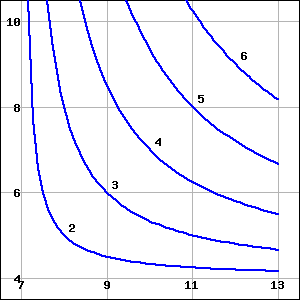
\includegraphics[width=0.75\textwidth]{fig/contour.png}
    \end{figure}
    The region we are considering is $R = [7,13]\times [4, 10]$.
    Using $\Delta x = \Delta y = 2$, find an overestimate and
    an underestimate for 
    $$\int_R f(x,y) \, dA.$$
    (Make sure to describe your process as well.)
\end{problem}

\begin{problem}
    The contour map shows the temperature in Fahrenheit at a certain time
    of a certain city in the US.
    Find an estimate of the average temperature of this city with $m =n=4$.
    \begin{figure}[!ht]
        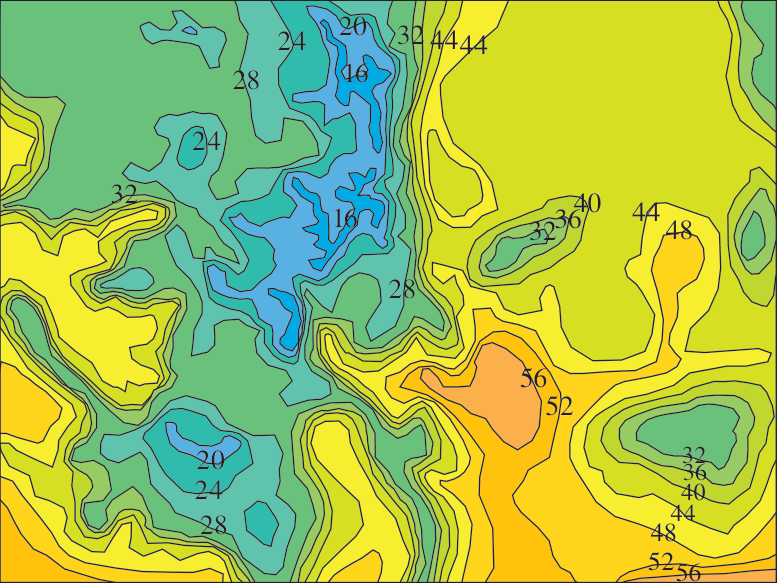
\includegraphics[width=0.75\textwidth]{fig/contour-temperature.png}
    \end{figure}
\end{problem}

\begin{problem}
    Calculate
    \begin{enumerate}
        \item $\iint_R x \sin (x+y) d A, \quad R=[0, \pi / 6] \times[0, \pi / 3]$
        \item $\iint_R \frac{x}{1+x y} d A, \quad R=[0,1] \times[0,1]$
        \item  $\iint_R y e^{-x y} d A, \quad R=[0,2] \times[0,3]$
        \item  $\iint_R \frac{1}{1+x+y} d A, \quad R=[1,3] \times[1,2]$
    \end{enumerate}
\end{problem}

\end{document}
